\documentclass{article}
%Packages%
\usepackage{geometry}
\geometry{a4paper,total={170mm,257mm},left=20mm,top=20mm}
\usepackage{titlesec}
\usepackage[english]{babel}
\usepackage[autostyle, english = american]{csquotes}
\usepackage{graphicx}
\MakeOuterQuote{"}

%Formatting%
\titleformat*{\section}{\bfseries\large}
\titleformat*{\subsection}{\bfseries\normalsize}

\title{Assignment 1: Second Stage}
\author{Go Uezono, Engi Takla, Melissa Aoko, Meenu Maheru}

\begin{document}
\maketitle

%------Q2------%
\section*{Question 2}
We will be using the instructor's solution for Question 1.

%------Q3------%
\section*{Question 3: Transition Diagram}
Recall that a string $\omega\in\Sigma\star$ belongs to $L$ if it satisfies \textbf{both} of the following conditions:
\begin{enumerate}
    \item The string "abad" is a substring of $\omega$.
    \item The string $\omega$ includes an even number of copies of the symbol "b".
\end{enumerate}
\noindent
Our deterministic finite automaton $M$ for the language $L$ is as follows: $$M=(Q,\Sigma,\delta,q_{\lambda,ev},F)$$ The components of $M$ include: \\
$Q: \{q_{\lambda,ev},q_{\lambda,od},q_{a,ev},q_{a,od},q_{ab,ev},q_{ab,od},q_{aba,ev},q_{aba,od},q_{abad,ev},q_{abad,od}\}$ - the finite, non-empty set of \textbf{states} \\
$\Sigma: \{a,b,c,d\}$ - the \textbf{alphabet} used to define the language $L$ \\
$\delta: Q \times \Sigma \rightarrow Q$ - the \textbf{transition function} of a well-defined function \\
$q_{\lambda,ev}$: the \textbf{start state} \\
$F: \{q_{abad,ev}\}$ - the set of \textbf{accepting state(s)}

\begin{center}
    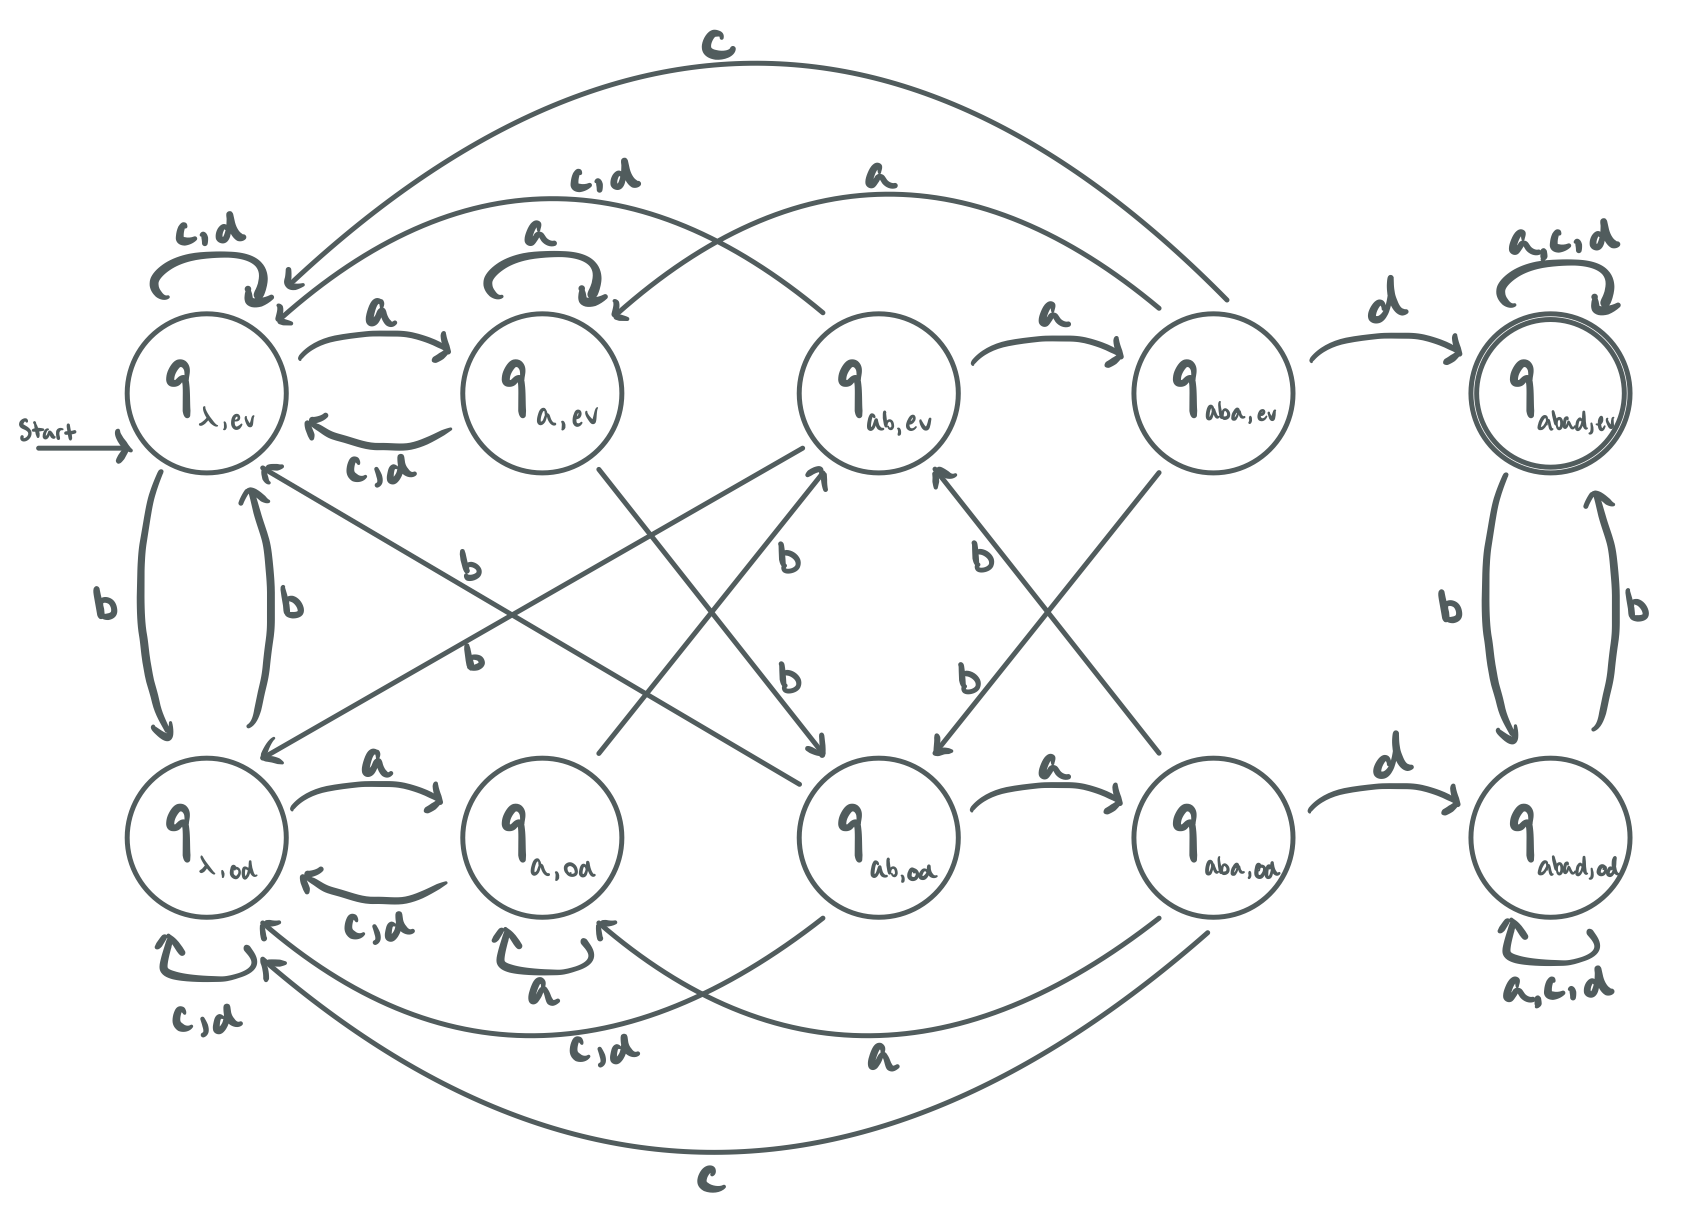
\includegraphics[width=\textwidth]{dfadiagram.png}
\end{center}

\newpage

%------Q4------%
\section*{Question 4: Prove that every string $\omega \in \Sigma \star$ belongs to exactly one of the subsets $S_q$ such that $q \in Q$.}

In order to prove every string $\omega \in \Sigma \star$ belongs to exactly one subset, $S_q$, such that $q \in Q$, we will use the technique, proof by exhaustion, to showcase all possible
cases for the string $\omega$. \\
As outlined in the deterministic finite automaton $M$ for the language $L$, we need to keep track of key components:
\begin{enumerate}
    \item Whether the string $\omega$ contains "abad" as a substring, and if it does not end with this, it must remember the longest prefix of "abad" that the string contains.
    \item Whether the string processed so far has an even or odd number of copies of "b".
\end{enumerate}
We will now prove that every string belongs to exactly \textbf{one} of the subsets $S_q$. There are 5 cases as we have outlined in the deterministic finite automaton to consider:

%--Case 1--%
\subsection*{Case 1: The string does not contain "abad" as a substring and does not end with "a", "ab", or "aba"}
\begin{itemize}
    \item If the string $\omega$ has no occurrence of "abad" as a substring and does not end with any prefix of "abad", this means that the deterministic finite automaton can only remain in the state $q_\lambda$.
    \item We must also consider the number of "b's" in the string $\omega$:
    \begin{itemize}
        \item If $\omega$ contains an even number of "b's", then $\omega \in S_{\lambda,ev}$
        \item If $\omega$ contains an odd number of "b's", then $\omega \in S_{\lambda,od}$ 
    \end{itemize}
    \item Therefore, the string can either belong to one of $S_{\lambda,ev}$ or $S_{\lambda,od}$, not both, depending on the number of copies of "b's" that have been proccessed in $\omega$.
\end{itemize}

%--Case 2--%
\subsection*{Case 2: The string does not contain "abad" as a substring but ends with "a"}
\begin{itemize}
    \item If the string $\omega$ does not have "abad" as a substring, but ends with "a", then the deterministic finite automaton must be in the state $q_a$.
    \item We must also consider the number of "b's" in the string $\omega$:
    \begin{itemize}
        \item If $\omega$ contains an even number of "b's", then $\omega \in S_{a,ev}$
        \item If $\omega$ contains an odd number of "b's", then $\omega \in S_{a,od}$  
    \end{itemize}
    \item Therefore, the string can either belong to one of $S_{a,ev}$ or $S_{a,od}$, not both, depending on the number of copies of "b's" that have been proccessed in $\omega$ so far.
\end{itemize}

%--Case 3--%
\subsection*{Case 3: The string does not contain "abad" as a substring but ends with "ab"}
\begin{itemize}
    \item If the string $\omega$ does not have the substring "abad" but ends with "ab", then the deterministic finite automaton must be in state $q_{ab}$.
    \item We must also consider the number of "b's" in the string $\omega$:
    \begin{itemize}
        \item If $\omega$ contains an even number of "b's", then $\omega \in S_{ab,ev}$
        \item If $\omega$ contains an odd number of "b's", then $\omega \in S_{ab,od}$  
    \end{itemize}
    \item Therefore, the string can either belong to one of $S_{ab,ev}$ or $S_{ab,od}$, not both, depending on the number of copies of "b's" that have been proccessed in $\omega$ so far.
\end{itemize}

%--Case 4--%
\subsection*{Case 4: The string does not contain "abad" as a substring but ends with "aba"}
\begin{itemize}
    \item If the string $\omega$ does not have the substring "abad" but ends with "aba", then the deterministic finite automaton must be in state $q_{aba}$.
    \item We must also consider the number of "b's" in the string $\omega$:
    \begin{itemize}
        \item If $\omega$ contains an even number of "b's", then $\omega \in S_{aba,ev}$
        \item If $\omega$ contains an odd number of "b's", then $\omega \in S_{aba,od}$  
    \end{itemize}
    \item Therefore, the string can either belong to one of $S_{aba,ev}$ or $S_{aba,od}$, not both, depending on the number of copies of "b's" that have been proccessed in $\omega$ so far.
\end{itemize}

%--Case 5--%
\subsection*{Case 5: The string contains "abad" as a substring}
\begin{itemize}
    \item If the string $\omega$ contains "abad" as a substring, then the deterministic finite automaton must be in state $q_{abad}$.
    \item We must also consider the number of "b's" in the string $\omega$:
    \begin{itemize}
        \item If $\omega$ contains an even number of "b's", then $\omega \in S_{abad,ev}$
        \item If $\omega$ contains an odd number of "b's", then $\omega \in S_{abad,od}$  
    \end{itemize}
    \item Therefore, the string can either belong to one of $S_{abad,ev}$ or $S_{abad,od}$, not both, depending on the number of copies of "b's" that have been proccessed in $\omega$ so far.
\end{itemize}

\noindent
Based on the above cases we have idenitfied, we have showed that every string $\omega \in \Sigma \star$ must belong to exactly \textbf{one} of the states in $L$. The above cases show that a string cannot 
belong to multiple states - a state cannot simultaneously contain and \textbf{not} contain the substring "abad", as well as simultaneously containing an even or odd number of "b's". It now follows that every 
string $\omega\in\Sigma\star$ of the language $L$ must belong to exactly \textbf{one} subset $S_q$. 
\newpage

%------Q5a------%
\section*{Question 5a: State all of the claims that you would need to include in a complete proof that the transition function for your DFA is well-defined.}
\begin{enumerate}
    \item $\{\omega\cdot a|\omega\in S_{\lambda,ev}\} \subseteq S_{a,ev}$, where $q_{a,ev}=\delta(q_{\lambda,ev},a)$
    \item $\{\omega\cdot b|\omega\in S_{\lambda,ev}\} \subseteq S_{\lambda,od}$, where $q_{\lambda,od}=\delta(q_{\lambda,ev},b)$
    \item $\{\omega\cdot c|\omega\in S_{\lambda,ev}\} \subseteq S_{\lambda,ev}$, where $q_{\lambda,ev}=\delta(q_{\lambda,ev},c)$
    \item $\{\omega\cdot d|\omega\in S_{\lambda,ev}\} \subseteq S_{\lambda,ev}$, where $q_{\lambda,ev}=\delta(q_{\lambda,ev},d)$
 
    \item $\{\omega\cdot a|\omega\in S_{\lambda,od}\} \subseteq S_{a,od}$, where $q_{a,od}=\delta(q_{\lambda,od},a)$
    \item $\{\omega\cdot b|\omega\in S_{\lambda,od}\} \subseteq S_{\lambda,ev}$, where $q_{\lambda,ev}=\delta(q_{\lambda,od},b)$
    \item $\{\omega\cdot c|\omega\in S_{\lambda,od}\} \subseteq S_{\lambda,od}$, where $q_{\lambda,od}=\delta(q_{\lambda,od},c)$
    \item $\{\omega\cdot d|\omega\in S_{\lambda,od}\} \subseteq S_{\lambda,od}$, where $q_{\lambda,od}=\delta(q_{\lambda,od},d)$
 
    \item $\{\omega\cdot a|\omega\in S_{a,ev}\} \subseteq S_{a,ev}$, where $q_{a,ev}=\delta(q_{a,ev},a)$
    \item $\{\omega\cdot b|\omega\in S_{a,ev}\} \subseteq S_{ab,od}$, where $q_{ab,od}=\delta(q_{a,ev},b)$
    \item $\{\omega\cdot c|\omega\in S_{a,ev}\} \subseteq S_{\lambda,ev}$, where $q_{\lambda,ev}=\delta(q_{a,ev},c)$
    \item $\{\omega\cdot d|\omega\in S_{a,ev}\} \subseteq S_{\lambda,ev}$, where $q_{\lambda,ev}=\delta(q_{a,ev},d)$
    
    \item $\{\omega\cdot a|\omega\in S_{a,od}\} \subseteq S_{a,od}$, where $q_{a,od}=\delta(q_{a,od},a)$
    \item $\{\omega\cdot b|\omega\in S_{a,od}\} \subseteq S_{ab,ev}$, where $q_{ab,ev}=\delta(q_{a,od},b)$
    \item $\{\omega\cdot c|\omega\in S_{a,od}\} \subseteq S_{\lambda,od}$, where $q_{\lambda,od}=\delta(q_{a,od},c)$
    \item $\{\omega\cdot d|\omega\in S_{a,od}\} \subseteq S_{\lambda,od}$, where $q_{\lambda,od}=\delta(q_{a,od},d)$
    
    \item $\{\omega\cdot a|\omega\in S_{ab,ev}\} \subseteq S_{aba,ev}$, where $q_{aba,ev}=\delta(q_{ab,ev},a)$
    \item $\{\omega\cdot b|\omega\in S_{ab,ev}\} \subseteq S_{\lambda,od}$, where $q_{\lambda,od}=\delta(q_{ab,ev},b)$
    \item $\{\omega\cdot c|\omega\in S_{ab,ev}\} \subseteq S_{\lambda,ev}$, where $q_{\lambda,ev}=\delta(q_{ab,ev},c)$
    \item $\{\omega\cdot d|\omega\in S_{ab,ev}\} \subseteq S_{\lambda,ev}$, where $q_{\lambda,ev}=\delta(q_{ab,ev},d)$
    
    \item $\{\omega\cdot a|\omega\in S_{ab,od}\} \subseteq S_{aba,od}$, where $q_{aba,od}=\delta(q_{ab,od},a)$
    \item $\{\omega\cdot b|\omega\in S_{ab,od}\} \subseteq S_{\lambda,ev}$, where $q_{\lambda,ev}=\delta(q_{ab,od},b)$
    \item $\{\omega\cdot c|\omega\in S_{ab,od}\} \subseteq S_{\lambda,od}$, where $q_{\lambda,od}=\delta(q_{ab,od},c)$
    \item $\{\omega\cdot d|\omega\in S_{ab,od}\} \subseteq S_{\lambda,od}$, where $q_{\lambda,od}=\delta(q_{ab,od},d)$
    
    \item $\{\omega\cdot a|\omega\in S_{aba,ev}\} \subseteq S_{a,ev}$, where $q_{a,ev}=\delta(q_{aba,ev},a)$
    \item $\{\omega\cdot b|\omega\in S_{aba,ev}\} \subseteq S_{ab,od}$, where $q_{ab,od}=\delta(q_{aba,ev},b)$
    \item $\{\omega\cdot c|\omega\in S_{aba,ev}\} \subseteq S_{\lambda,ev}$, where $q_{\lambda,ev}=\delta(q_{aba,ev},c)$
    \item $\{\omega\cdot d|\omega\in S_{aba,ev}\} \subseteq S_{abad,ev}$, where $q_{abad,ev}=\delta(q_{aba,ev},d)$
    
    \item $\{\omega\cdot a|\omega\in S_{aba,od}\} \subseteq S_{a,od}$, where $q_{a,od}=\delta(q_{aba,od},a)$
    \item $\{\omega\cdot b|\omega\in S_{aba,od}\} \subseteq S_{ab,ev}$, where $q_{ab,ev}=\delta(q_{aba,od},b)$
    \item $\{\omega\cdot c|\omega\in S_{aba,od}\} \subseteq S_{\lambda,od}$, where $q_{\lambda,od}=\delta(q_{aba,od},c)$
    \item $\{\omega\cdot d|\omega\in S_{aba,od}\} \subseteq S_{abad,od}$, where $q_{abad,od}=\delta(q_{aba,od},d)$
    
    \item $\{\omega\cdot a|\omega\in S_{abad,ev}\} \subseteq S_{abad,ev}$, where $q_{abad,ev}=\delta(q_{abad,ev},a)$
    \item $\{\omega\cdot b|\omega\in S_{abad,ev}\} \subseteq S_{abad,od}$, where $q_{abad,od}=\delta(q_{abad,ev},b)$
    \item $\{\omega\cdot c|\omega\in S_{abad,ev}\} \subseteq S_{abad,ev}$, where $q_{abad,ev}=\delta(q_{abad,ev},c)$
    \item $\{\omega\cdot d|\omega\in S_{abad,ev}\} \subseteq S_{abad,ev}$, where $q_{abad,ev}=\delta(q_{abad,ev},d)$
    
    \item $\{\omega\cdot a|\omega\in S_{abad,od}\} \subseteq S_{abad,od}$, where $q_{abad,od}=\delta(q_{abad,od},a)$
    \item $\{\omega\cdot b|\omega\in S_{abad,od}\} \subseteq S_{abad,ev}$, where $q_{abad,ev}=\delta(q_{abad,od},b)$
    \item $\{\omega\cdot c|\omega\in S_{abad,od}\} \subseteq S_{abad,od}$, where $q_{abad,od}=\delta(q_{abad,od},c)$
    \item $\{\omega\cdot d|\omega\in S_{abad,od}\} \subseteq S_{abad,od}$, where $q_{abad,od}=\delta(q_{abad,od},d)$
\end{enumerate}

%------Q5b------%
\section*{Question 5b: Prove all the claims that are needed to establish that the transitions out of the start state, $q_{\lambda,ev}$, are well-defined.}
Let us first define our start state, $S_{\lambda,ev}$:
\begin{center}
    $S_{\lambda,ev}=$\{$\omega\in\Sigma\star|\omega$ does not have "abad" as a substring and does not end with either "a" or "ab", and $\omega$ includes an even number of copies of "b" \}
\end{center}

%--Claim 1--%
\subsection*{Claim 1: $\{\omega\cdot a|\omega\in S_{\lambda,ev}\} \subseteq S_{a,ev}$}
\begin{itemize}
    \item As mentioned above, the string $\omega$ does not contain the substring "abad", and "a" or "ab", and contains an even number of "b". When our deterministic finite automaton reads the string "a", then 
    the new string $\omega\cdot a$ ends with an "a". The resulting string does not contain "abad" as a substring, it ends with an "a" but not "aba", and the number of "b's" remain unchanged,
    which is even - thus, $\omega$ fits the definition of $S_{a,ev}$, so that $\omega\cdot a\in S_{a,ev}$. 
    \item Since $\omega$ was arbitrarily chosen from $S_{\lambda,ev}$, it follows that $\{\omega\cdot a|\omega\in S_{\lambda,ev}\}\subseteq S_{a,ev}$ 
\end{itemize}

%--Claim 2--%
\subsection*{Claim 2: $\{\omega\cdot b|\omega\in S_{\lambda,ev}\} \subseteq S_{\lambda,od}$}
\begin{itemize}
    \item The string $\omega$ does not contain the substring "abad", and "a" or "ab", and contains an even number of "b". When our deterministic finite automaton reads the string "b", then 
    the new string $\omega\cdot b$ ends with a "b". The resulting string does not contain "abad" as a substring, does not end with an "a" or "ab", and the number of "b's" become odd - thus, $\omega$ fits the 
    definition of $S_{\lambda,od}$, so that $\omega\cdot b\in S_{\lambda,od}$. 
    \item Since $\omega$ was arbitrarily chosen from $S_{\lambda,ev}$, it follows that $\{\omega\cdot b|\omega\in S_{\lambda,ev}\}\subseteq S_{\lambda,od}$ 
\end{itemize}

%--Claim 3--%
\subsection*{Claim 3: $\{\omega\cdot c|\omega\in S_{\lambda,ev}\} \subseteq S_{\lambda,ev}$}
\begin{itemize}
    \item The string $\omega$ does not contain the substring "abad", and "a" or "ab", and contains an even number of "b". When our deterministic finite automaton reads the string "c", then 
    the new string $\omega\cdot c$ ends with a "c". The resulting string does not contain "abad" as a substring, does not end with an "a" or "ab", and the number of "b's" remain unchanged, which is even - 
    thus, $\omega$ fits the definition of $S_{\lambda,ev}$, so that $\omega\cdot c\in S_{\lambda,ev}$. 
    \item Since $\omega$ was arbitrarily chosen from $S_{\lambda,ev}$, it follows that $\{\omega\cdot c|\omega\in S_{\lambda,ev}\}\subseteq S_{\lambda,ev}$ 
\end{itemize}
%--Claim 4--%
\subsection*{Claim 4: $\{\omega\cdot d|\omega\in S_{\lambda,ev}\} \subseteq S_{\lambda,ev}$}
\begin{itemize}
    \item The string $\omega$ does not contain the substring "abad", and "a" or "ab", and contains an even number of "b". When our deterministic finite automaton reads the string "d", then 
    the new string $\omega\cdot d$ ends with a "d". The resulting string does not contain "abad" as a substring, does not end with an "a" or "ab", and the number of "b's" remain unchanged, which is even - 
    thus, $\omega$ fits the definition of $S_{\lambda,ev}$, so that $\omega\cdot d\in S_{\lambda,ev}$. 
    \item Since $\omega$ was arbitrarily chosen from $S_{\lambda,ev}$, it follows that $\{\omega\cdot d|\omega\in S_{\lambda,ev}\}\subseteq S_{\lambda,ev}$ 
\end{itemize}
\noindent
Since all of the transitions out of the start state $q_{\lambda,ev}$ are defined for all symbols $\sigma\in\Sigma$, we conclude that the start state $q_{\lambda,ev}$ is well-defined.
\newpage

%------Q6------%
\section*{Question 6: State, and prove, all of the other claims (involving the sets $S_q \subseteq \Sigma\star$ for states, $q$, in your determinstic finite automaton)
that you would need to include in a proof that $L$ is the language of your deterministic finite automaton. (Yes: You need to establish more than the fact that 
"the transition function is well-defined.")}

To answer this question, we must recall what our definition of $L$ is. In order for $L$ to accept a string, the following conditions (both) must be satisfied: 1) The 
string "abad" is a substring of $\omega$; and 2) The string $\omega$ includes an even number of the symbol "b". Since we have proven the transition functions to be well-defined
earlier, the following claims must be proven:

%--Claim 1--%
\subsection*{Claim 1: $\lambda \in S_{\lambda,ev}$}
\begin{itemize}
    \item Suppose we have an empty string $\lambda$. A string belongs to the set $S_{\lambda,ev}$ if "abad" is not a substring, does not end with either "a" or "ab", and 
    the string contains an even copies of "b". By definition, the empty string $\lambda$ contains no symbols (string of length zero), and having 0 copies of the symbol "b" is 
    considered even, thus it does not contain any symbols whatsoever. Hence, $\lambda$ fits the definition of $S_{\lambda,ev}$, so it follows that $\lambda \in S_{\lambda,ev}$ as claimed.
\end{itemize}

%--Claim 2--%
\subsection*{Claim 2: $S_{\lambda,ev} \cap L = \emptyset$, $S_{\lambda,od} \cap L = \emptyset$, $S_{a,ev} \cap L = \emptyset$, $S_{a,od} \cap L = \emptyset$, $S_{ab,ev} \cap L = \emptyset$, 
$S_{ab,od} \cap L = \emptyset$, $S_{aba,ev} \cap L = \emptyset$, $S_{aba,od} \cap L = \emptyset$, and $S_{abad,od} \cap L = \emptyset$ such that $q_{\lambda,ev} \notin F$, $q_{\lambda,od} \notin F$, 
$q_{a,ev} \notin F$, $q_{a,od} \notin F$, $q_{ab,ev} \notin F$, $q_{ab,od} \notin F$, $q_{aba,ev} \notin F$, $q_{aba,od} \notin F$, and $q_{abad,od} \notin F$}
\begin{itemize}
    \item Let $\omega \in S_{\lambda,ev}$. By the definition of $S_{\lambda,ev}$, it follows that a string belongs to this set if it does not contain the substring "abad", does not end with "a" or "ab",
    and includes an even number of "b's". Although $\omega$ satisfies the 2) condition of $L$ (contains an even number of "b's"), it does not contain the substring "abad". Since only one of the two conditions 
    were met, $\omega \notin L$ and since $\omega$ was arbitrarily chosen from $S_{\lambda,ev}$, it follows that $\omega \notin L$ for all $\omega \in S_{\lambda,ev}$ - thus, $S_{\lambda,ev} \cap L = \emptyset$
    as claimed.

    \item Let $\omega \in S_{\lambda,od}$. By the definition of $S_{\lambda,od}$, it follows that a string belongs to this set if it does not contain the substring "abad", does not end with "a" or "ab",
    and includes an odd number of "b's". $\omega$ does not contain the subtring "abad", which is unaligned with the 1) condition, and it contains an odd number of "b's", which is unaligned with the 2) condition.
    Since none of the conditions were met, $\omega \notin L$ and since $\omega$ was arbitrarily chosen from $S_{\lambda,od}$, it follows that $\omega \notin L$ for all $\omega \in S_{\lambda,od}$ - thus, 
    $S_{\lambda,od} \cap L = \emptyset$ as claimed.

    \item Let $\omega \in S_{a,ev}$. By the definition of $S_{a,ev}$, it follows that a string belongs to this set if it does not contain the substring "abad", ends with "a" but not "aba",
    and includes an even number of "b's". Although $\omega$ satisfies the 2) condition of $L$ (contains an even number of "b's"), it does not contain the substring "abad". Since only one of the two conditions 
    were met, $\omega \notin L$ and since $\omega$ was arbitrarily chosen from $S_{a,ev}$, it follows that $\omega \notin L$ for all $\omega \in S_{a,ev}$ - thus, $S_{a,ev} \cap L = \emptyset$
    as claimed.

    \item Let $\omega \in S_{a,od}$. By the definition of $S_{a,od}$, it follows that a string belongs to this set if it does not contain the substring "abad", ends with "a" but not "aba",
    and includes an odd number of "b's". $\omega$ does not contain the subtring "abad", which is unaligned with the 1) condition, and it contains an odd number of "b's", which is unaligned with the 2) condition.
    Since none of the conditions were met, $\omega \notin L$ and since $\omega$ was arbitrarily chosen from $S_{a,od}$, it follows that $\omega \notin L$ for all $\omega \in S_{a,od}$ - thus, $S_{a,od} \cap L = \emptyset$
    as claimed.

    \item Let $\omega \in S_{ab,ev}$. By the definition of $S_{ab,ev}$, it follows that a string belongs to this set if it does not contain the substring "abad", ends with "ab", and includes an even number of "b's". 
    Although $\omega$ satisfies the 2) condition of $L$ (contains an even number of "b's"), it does not contain the substring "abad". Since only one of the two conditions were met, $\omega \notin L$ and since $\omega$ 
    was arbitrarily chosen from $S_{ab,ev}$, it follows that $\omega \notin L$ for all $\omega \in S_{ab,ev}$ - thus, $S_{ab,ev} \cap L = \emptyset$ as claimed.

    \item Let $\omega \in S_{ab,od}$. By the definition of $S_{ab,od}$, it follows that a string belongs to this set if it does not contain the substring "abad", ends with "ab", and includes an odd number of "b's". 
    $\omega$ does not contain the subtring "abad", which is unaligned with the 1) condition, and it contains an odd number of "b's", which is unaligned with the 2) condition. Since none of the conditions were met, 
    $\omega \notin L$ and since $\omega$ was arbitrarily chosen from $S_{ab,od}$, it follows that $\omega \notin L$ for all $\omega \in S_{ab,od}$ - thus, $S_{ab,od} \cap L = \emptyset$ as claimed.

    \item Let $\omega \in S_{aba,ev}$. By the definition of $S_{aba,ev}$, it follows that a string belongs to this set if it does not contain the substring "abad", ends with "ab", and includes an even number of "b's". 
    Although $\omega$ satisfies the 2) condition of $L$ (contains an even number of "b's"), it does not contain the substring "abad". Since only one of the two conditions were met, $\omega \notin L$ and since $\omega$ 
    was arbitrarily chosen from $S_{aba,ev}$, it follows that $\omega \notin L$ for all $\omega \in S_{aba,ev}$ - thus, $S_{aba,ev} \cap L = \emptyset$ as claimed.

    \item Let $\omega \in S_{aba,od}$. By the definition of $S_{aba,od}$, it follows that a string belongs to this set if it does not contain the substring "abad", ends with "aba", and includes an odd number of "b's". 
    $\omega$ does not contain the subtring "abad", which is unaligned with the 1) condition, and it contains an odd number of "b's", which is unaligned with the 2) condition. Since none of the conditions were met, 
    $\omega \notin L$ and since $\omega$ was arbitrarily chosen from $S_{aba,od}$, it follows that $\omega \notin L$ for all $\omega \in S_{aba,od}$ - thus, $S_{aba,od} \cap L = \emptyset$ as claimed.

    \item Let $\omega \in S_{abad,od}$. By the definition of $S_{abad,od}$, it follows that a string belongs to this set if it contains the substring "abad" and includes an odd number of "b's". 
    Although $\omega$ includes the substring "abad" - which satisfies the 1) condition - it contains an odd number of "b's", which does not satisfy the 2) condition. Since only the one of the two conditions were met, 
    $\omega \notin L$ and since $\omega$ was arbitrarily chosen from $S_{abad,od}$, it follows that $\omega \notin L$ for all $\omega \in S_{abad,od}$ - thus, $S_{abad,od} \cap L = \emptyset$ as claimed.

    \item With the above claims proved, it follows that $S_{\lambda,ev} \cap L = \emptyset$, $S_{\lambda,od} \cap L = \emptyset$, $S_{a,ev} \cap L = \emptyset$, $S_{a,od} \cap L = \emptyset$, $S_{ab,ev} \cap L = \emptyset$, 
    $S_{ab,od} \cap L = \emptyset$, $S_{aba,ev} \cap L = \emptyset$, $S_{aba,od} \cap L = \emptyset$, and $S_{abad,od} \cap L = \emptyset$, such that $q_{\lambda,ev} \notin F$, $q_{\lambda,od} \notin F$, 
    $q_{a,ev} \notin F$, $q_{a,od} \notin F$, $q_{ab,ev} \notin F$, $q_{ab,od} \notin F$, $q_{aba,ev} \notin F$, $q_{aba,od} \notin F$, and $q_{abad,od} \notin F$, as claimed.
\end{itemize}
%--Claim 3--%
\subsection*{Claim 3: $S_{abad,ev} \subseteq L$ such that $q_{abad,ev} \in F$}
\begin{itemize}
    \item Let $\omega \in S_{abad,ev}$. By the definition of $S_{abad,ev}$, it follows that $\omega$ contains the substring "abad" AND an even number of "b's", which satisfies conditions 
    1) and 2). Then, $\omega$ meets both of the conditions of $L$, so we conclude that $\omega \in L$. Since $\omega$ was arbitrarily chosen from $S_{abad,ev}$, it follows that $S_{abad,ev} \subseteq L$
    , such that $q_{abad,ev} \in F$.
\end{itemize}

\noindent
Since the claims 1, 2, and 3 are satisfied, we have proven that the transition function is well-defined. By the theorem of the "correctness of a DFA" from the lecture notes, it now follows that the language $L(M) = L$, 
as claimed.

\end{document}